\section{Cathode}

In a Hall Thruster, a cathode serves two primary functions. The first is to provide the electrons that are used to create the Hall current, which ionize the neutral propellant injected from the anode. The second function is to provide the electrons that are injected into the thruster plume, which neutralizes the ions in the plume. This prevents the induction of a potential difference between the plume and thruster that would attract the ion back into the thruster \cite{AIAA2008-5188}. 

The placement of the cathode is an important factor that affects plume characteristics, which by extension affects thruster efficiency, among other things. The two most common concepts for placing the cathode are mounting it inside the chamber, along the central axis of the the thruster, or mounting it externally, outside the thruster body. Characteristics of both mounting methods are discussed below.

\subsection{Externally Mounted Cathode}

Externally mounted cathodes are the most common configuration found in \ac{HET}'s. The cathode is placed downstream of the thruster plane, as seen in the figure below.. 

\begin{figure}[H]
    \centering
    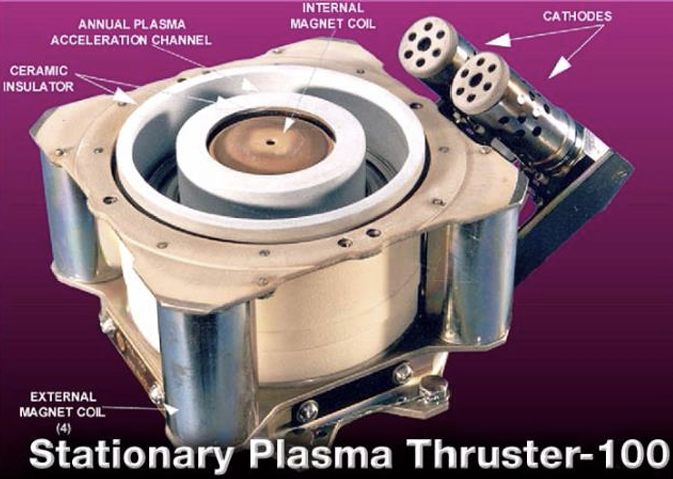
\includegraphics[width=0.7\textwidth]{images/Concepts/ExternalCathode.png}
    \captionsetup{justification=centering}
    \caption{\ac{HET} with an Externally Mounted Cathode \cite{ExternalCathodePic}}
    \label{fig:external_cathode}
\end{figure}

There are clear benefits to mounting the cathode externally. Having the cathode externally mounted makes it easier to test, troubleshoot and replace (during testing), allowing for a more modular design. It also reduces the complexity of the architecture inside the thruster channel, since considerations for integrating the cathode and managing its thermal requirements and effects would not be an issue \cite{nasajpltext}.

Having the cathode mounted externally and radially has its disadvantages as well. The offset eletron stream, both into the chamber and to neutralize the plume, leads to assymetrical plume characteristics reduced current utlization, both of which reduce thruster efficiency \cite{nasajpltext}.

\subsection{Centrally Mounted Cathode}

A centrally mounted cathode is often integrated inside the inner magnetic core, at the center of the thruster chamber. Having a centrally mounted cathode is highly advantageous since the symmetric electron injection allows for more uniform plume characteristics. The figure below depicts the architecture of a Hall thruster with a centrally mounted cathode \cite{nasajpltext}. 

\begin{figure}[H]
    \centering
    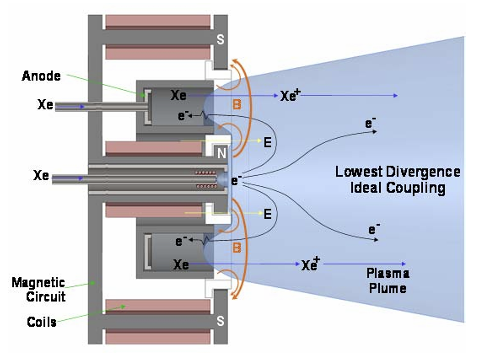
\includegraphics[width=0.7\textwidth]{images/Concepts/CentralCathode.png}
    \captionsetup{justification=centering}
    \caption{An Axisymmetric \ac{HET} geometry with a Center Mounted Cathode \cite{CentralCathodePic}}
    \label{fig:center_mounter_cathode}
\end{figure}

A centrally mounted cathode, when done correctly, results in improved thruster performance relative to a one with an externally mounted cathode. However, getting a centrally mounted cathode right requires careful tuning of the magnetic field lines and greater consideration to structural integration. There is also the added complexity of dealing with the thermal and mechanical interactions of the cathode in the chamber \cite{nasajpltext}.

Other than placement of the cathode, the type of cathode to be used also needs to be considered. The two most common types of cathodes are thermionic cathodes and hollow cathodes. 

% Thermionic cathodes work by heating up a filament, usually tungsten or another refractory metal, up to extremely high temperatures, which causes electrons to be emitted directly from its surface. In contrast, hollow cathodes consist of a cylindrical tube which contains a low work-function insert, such as barium-oxide coated tungsten, a heater and a keeper electrode. This insert emits electrons at lower temperatures relative to a thermionic cathode, and further internal plasma interactions enhance electron emissions beyond thermionic processes \cite{nasagrc}.   

Hollow cathodes are hence more efficient than thermionic cathodes, since the low temperature requirement results in a lower power draw. The low temperature requirement and higher electron emission also allows for easier and more generous integration considerations for a centrally mounted cathode \cite{nasajpltext}. 